% Exemplo de relatório técnico do IC
% Criado por P.J.de Rezende antes do Alvorecer da História.
% Modificado em 97-06-15 e 01-02-26 por J.Stolfi.
% Last edited on 2003-06-07 21:12:18 by stolfi
% modificado em 1o. de outubro de 2008
% modificado em 2012-09-25 para ajustar o pacote UTF8. Contribuicao de
%   Rogerio Cardoso

\documentclass[11pt,twoside]{article}
\usepackage{techrep-ic}
\usepackage{indentfirst}

%%% SE USAR INGLÊS, TROQUE AS ATIVAÇÕES DOS DOIS COMANDOS A SEGUIR:
\usepackage[brazil]{babel}
%% \usepackage[english]{babel}

%%% SE USAR CODIFICAÇÃO LATIN1, TROQUE AS ATIVAÇÕES DOS DOIS COMANDOS A
%%% SEGUIR:
%% \usepackage[latin1]{inputenc}
\usepackage[utf8]{inputenc}
\usepackage{graphicx}

\begin{document}

%%% PÁGINA DE CAPA %%%%%%%%%%%%%%%%%%%%%%%%%%%%%%%%%%%%%%%%%%%%%%%
%
% Número do relatório
\TRNumber{02}

% DATA DE PUBLICAÇÃO (PARA A CAPA)
%
\TRYear{16}  % Dois dígitos apenas
\TRMonth{04} % Numérico, 01-12

% LISTA DE AUTORES PARA CAPA (sem afiliações).
\TRAuthor{Gabriel Oliveira \and Jo{\~a}o Fid{\'e}lis \and Lucas Morais \and Matheus Figueiredo \and Pedro Grij{\'o}}

% TÍTULO PARA A CAPA (use \\ para forçar quebras de linha).
\TRTitle{MC437 - Grupo06 - Relat{\'o}rio 2}

\TRMakeCover
%%%%%%%%%%%%%%%%%%%%%%%%%%%%%%%%%%%%%%%%%%%%%%%%%%%%%%%%%%%%%%%%%%%%%%
% O que segue é apenas uma sugestão - sinta-se à vontade para
% usar seu formato predileto, desde que as margens tenham pelo
% menos 25mm nos quatro lados, e o tamanho do fonte seja pelo menos
% 11pt. Certifique-se também de que o título e lista de autores
% estão reproduzidos na íntegra na página 1, a primeira depois da
% página de capa.
%%%%%%%%%%%%%%%%%%%%%%%%%%%%%%%%%%%%%%%%%%%%%%%%%%%%%%%%%%%%%%%%%%%%%%

%%%%%%%%%%%%%%%%%%%%%%%%%%%%%%%%%%%%%%%%%%%%%%%%%%%%%%%%%%%%%%%%%%%%%%
% Nomes de autores ABREVIADOS e titulo ABREVIADO,
% para cabeçalhos em cada página.
%
\markboth{Bueno, Fid{\'e}lis, Figueiredo, Grij{\'o}, Morais}{MC437 - Grupo06}
\pagestyle{myheadings}

%%%%%%%%%%%%%%%%%%%%%%%%%%%%%%%%%%%%%%%%%%%%%%%%%%%%%%%%%%%%%%%%%%%%%%
% TÍTULO e NOMES DOS AUTORES, completos, para a página 1.
% Use "\\" para quebrar linhas, "\and" para separar autores.
%
\title{MC437 - Grupo06}

\author{Gabriel Bueno de Oliveira \and
Jo{\~a}o Guilherme Daros Fid{\'e}lis \and
Lucas Henrique Morais \and
Matheus Yokoyama Figueiredo \and Pedro Rodrigues Grij{\'o}}
\date{}

\maketitle

%%%%%%%%%%%%%%%%%%%%%%%%%%%%%%%%%%%%%%%%%%%%%%%%%%%%%%%%%%%%%%%%%%%%%%

\begin{abstract}
\setlength{\parindent}{4ex}
Utilizamos o benchmark TPC-W, que modela uma livraria online, atrav\'es de um ambiente controlado, para simular atividades num servidor WEB. Em conjunto com o simulador RBE, que gera tr\^es diferentes perfis de carga (Shopping, Ordering e Browsing), pudemos checar o desempenho do servidor instalado num cluster no IC, ao vermos o n\'umero de WIPS (WEB Interactions per Second) gerados por diferentes cargas.
O relat\'orio refere-se a segunda parte do projeto da disciplina de MC437 (Projeto de Sistemas de Informa\c{c}\~ao) e tem como objetivo realizar testes com dois bancos de dados diferentes, sendo um primário que é replicado para um secundário em hot-standby, testando quais as melhores cargas que o primário consegue atender e depois medir o tempo de recuperação quando o primário é desligado e o secundário promovido.
\end{abstract}

\section{Introdução}
Este trabalho \'e um relat\'orio da segunda parte do projeto da displina, que consistiu em preparar além da m\'aquina remota com o servidor Tomcat, utlizar duas máquinas desse cluster com instâncias do PostgreSQL, uma com um banco de dados atuando como primário e outra atuando como um banco secundário em hot-standby para integrar todas essas funcionalidades e fazer um site de compras com dados gerados aleatoriamente.

    Também foi instalado na máquina o aplicativo TPC-W que \'e um benchmark de transa\c{c}\~oes web, que é uma aplica\c{c}\~ao Java. Para utilizar o TPC-W, foi utlizado o RBE (Remote Browser Emulator), que emula conjuntos de clientes que acessam o lado servidor do TPC-W, que implementa uma loja de livros.

    O RBE \'e um simulador escrito completamente em Java que simula o tr\'afego HTTP que seria feito por um usu\'ario que estivesse acessando o site atrav\'es de um navegador.

    Também utilizamos o HAProxy, que atua como um proxy para aplicações baseadas em TCP e HTTP. Ele oferece alta disponibilidade e balanceamento de carga para servidores web. Sua função nesse trabalho é assim que detectar que o banco primário falhou, redirecionar as requisições feitas para o antigo banco secndário que deve ser promovido a banco primário.

    O TPC-W gera um n\'umero, o WIPS (Web Interactions per Second, n\'umero de itera\c{c}\~oes Web por segundo). O fluxo de trabalho é gerado pelo RBE e pode ser de tr\^es tipos diferentes de perfis. O perfil de compras (\textit{shopping}), onde 80\% das a\c{c}\~oes são de consulta e 20\% de escrita no banco de dados. O perfil de navega\c{c}\~ao (\textit{browsing}), tem 95\% das a\c{c}\~oes de leitura e 5\% de escrita. J\'a o perfil de compras (\textit{ordering}) tem metades de suas opera\c{c}\~oes de leitura e a outra metade de escrita.

    Rodamos três experimentos diferentes, o primeiro apenas com o banco primário ativo, o segundo com o primário ligado e o secundário ligado em hot-standby e o terceiro onde na metade do experimento, o primário era desativado para que o secundário pudesse ser promovido.

\setlength{\parindent}{4ex}


\section{Condições Experimentais}
\setlength{\parindent}{4ex}
     Nesta se\c{c}\~ao ser\~ao descritas as configura\c{c}\~oes de hardware e software utilizadas nos experimentos.

     Nesta fase, contamos com quatro máquinas, todas iguais e fornecidas pelo Instituto de computação.

     A primeira, chamada CBN6, é onde está instalado o HAProxy X.XX, Tomcat versão 7 e TPC-W. Ela que atua como servidor web.

     Duas máquinas, a dbmaster2 e dbslave2, é onde ficam os banco de dados primário e secundário, respectivamente. Também tem instalados o PostgreSQL vers\~ao 9.5.1.

     Já o RBE foi rodado a partir de outra máquina, a CBN 7.

     Todas as máquinas tem a mesma configuração: sistema operacional Ubuntu 14.04, CPU Intel(R) Core(TM)2 Quad CPU Q8400 2.66GHz e mem\'oria RAM de 4GB e 1333 MHz.

\section{Metodologia de Pesquisa}
\setlength{\parindent}{4ex}
Foi necessário executar três diferentes experimentos. Cada experimento consiste em rodar o RBE para simular uma carga no servidor e avaliarmos as medições feitas.

O primeiro experimento, foi utilizar o RBE com apenas o banco primário ligado. No segundo experimento, estavam ligados os bancos primários e o secundário em hot-standby.

Esses dois experimentos, são feitos para caracterizar nosso servidor. O objetivo é medir a maior carga para a qual ele se comporta de forma consistente.

Para isso, variamos os valores de carga entre 2000 e 4000 clientes, variando de 1000 em cada iteração, isso para cada perfil de usuário descrito anteriormente. Assim, podemos fazer gráficos que nos mostram até qual carga o servidor manteve um bom nível de WIPS ao longo de todo o teste (que dura 100s no total).

Com esse valor achado, utilizamos esse valor de carga e utilizamos o RBE para simular essa "carga ótima" no servidor, causando um failover  manualmente (isto é, matando o banco de dados primário), enquanto promovemos o banco de dados secundário, para ver em quanto tempo nosso servidor consegue se recuperar e voltar a ficar ativo.

É importante ressaltar que sempre rodamos o RBE de outra máquina remota (CBN7), diferente de nosso servidor, e que os parâmetros utilizados foram Ramp-Up Time: 5s, Ramp-Down Time: 5s e Measurement Interval: 90s. O valor de máximo número de erros tolerados foi colocado em 0. Todos os outros valores são os padrões do RBE.

\section{An\'alise e Resultados}
\setlength{\parindent}{4ex}

Seguem os gráficos gerados pela execução do RBE para cada experimento.
\begin{center}
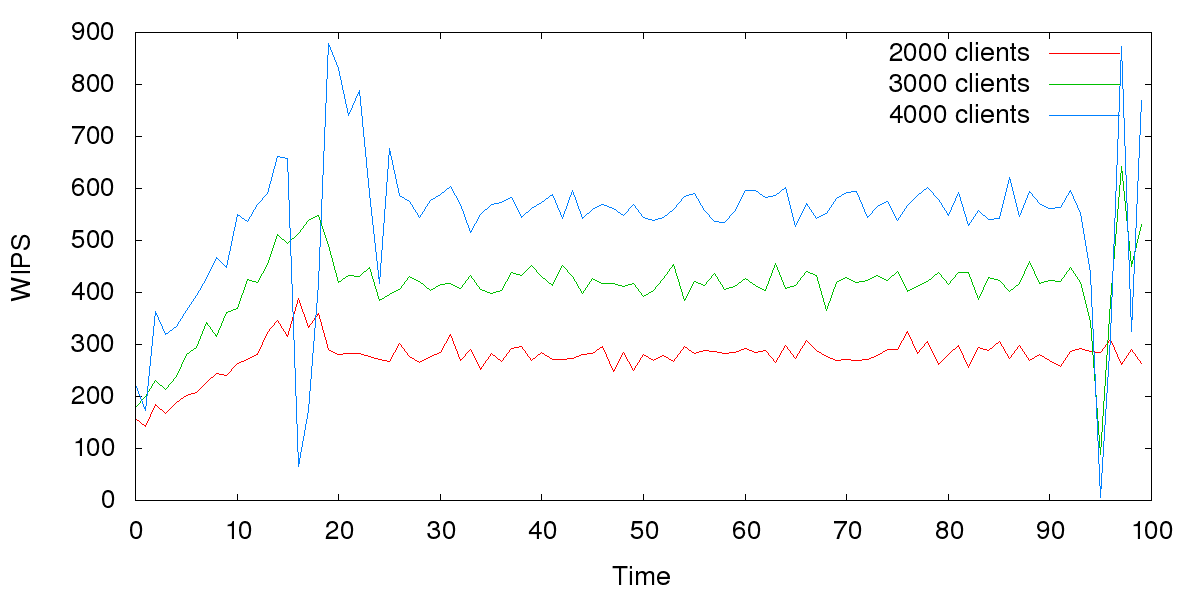
\includegraphics[width=15cm, height=10cm]{images/exp1/plot_browsin}
Figura 1: WIPSb por tempo para cada carga simulada pelo RBE no perfil Browsing no experimento 1
\end{center}
Vemos que 4000 usuários teve uma boa consistência durante o meio do experimento mas uma grande queda no final, assim como o de 3000. O de 4000 também houve uma variação grande por volta dos 15 segundos.
\begin{center}
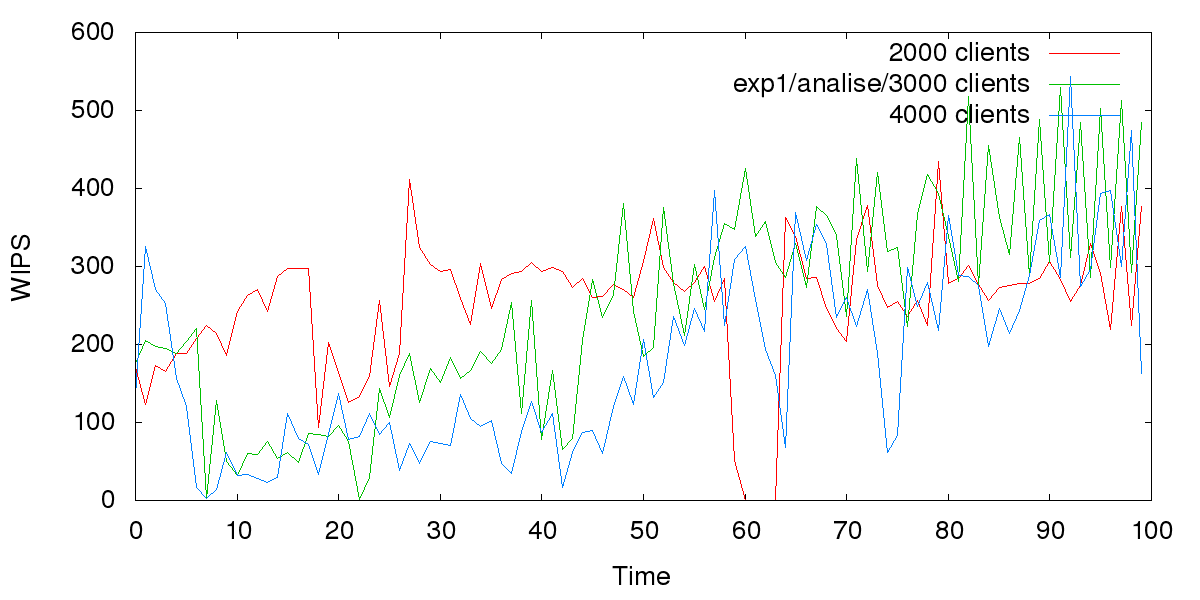
\includegraphics[width=15cm, height=10cm]{images/exp1/plot_ordering}
Figura 2: WIPSo por tempo para cada carga simulada pelo RBE no perfil Ordering no experimento 1
\end{center}
Pelo gráfico, podemos ver que oteste com 3000 clientes teve o melhor desempenho no geral. Até a metade, 2000 usuários estava melhor mas depois 3000 foi crescendo e manteve uma boa taxa até o final.
\begin{center}
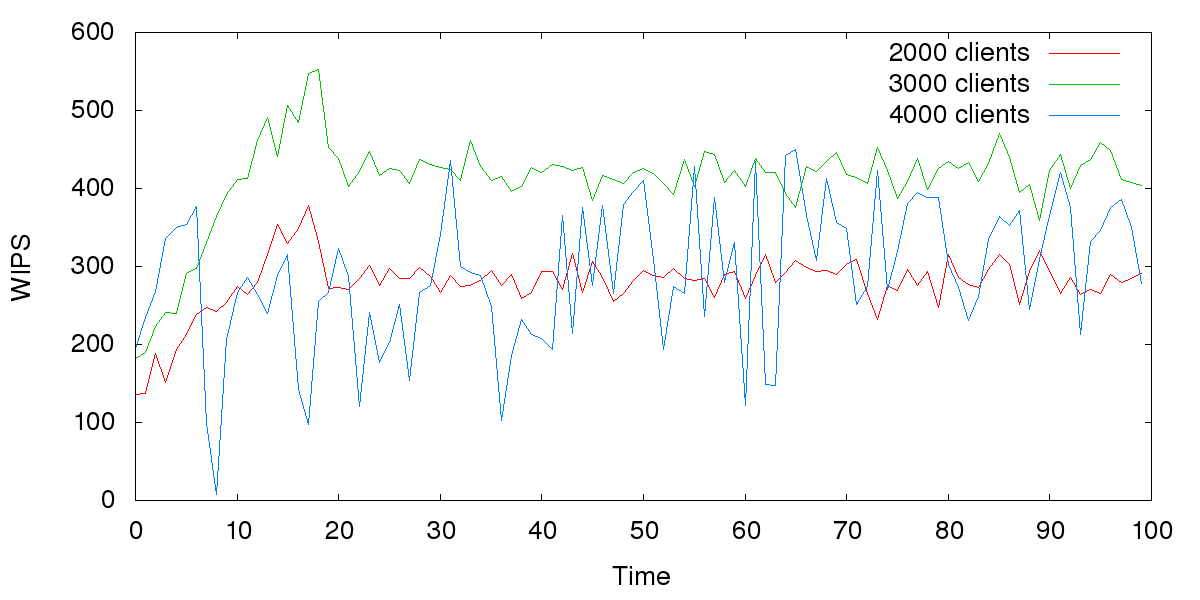
\includegraphics[width=15cm, height=10cm]{images/exp1/plot_shopping}
Figura 3: WIPS por tempo para cada carga simulada pelo RBE no perfil Shopping no experimento 1
\end{center}

Neste gráfico, ficou evidente o melhor desempenho da simulação com 3000 clientes sobre as duas outras. Uma melhor taxa de WIPS foi obtida durante praticamente todo o experimento.

Esses três gráficos combinados, nos dá indícios de que 3000 usuários talvez seja o melhor número a ser utilizado, pois tem taxas de WIPS mais altas e estáveis que as outras testadas.

Agora, analisaremos os dados do experimento 2.

\begin{center}
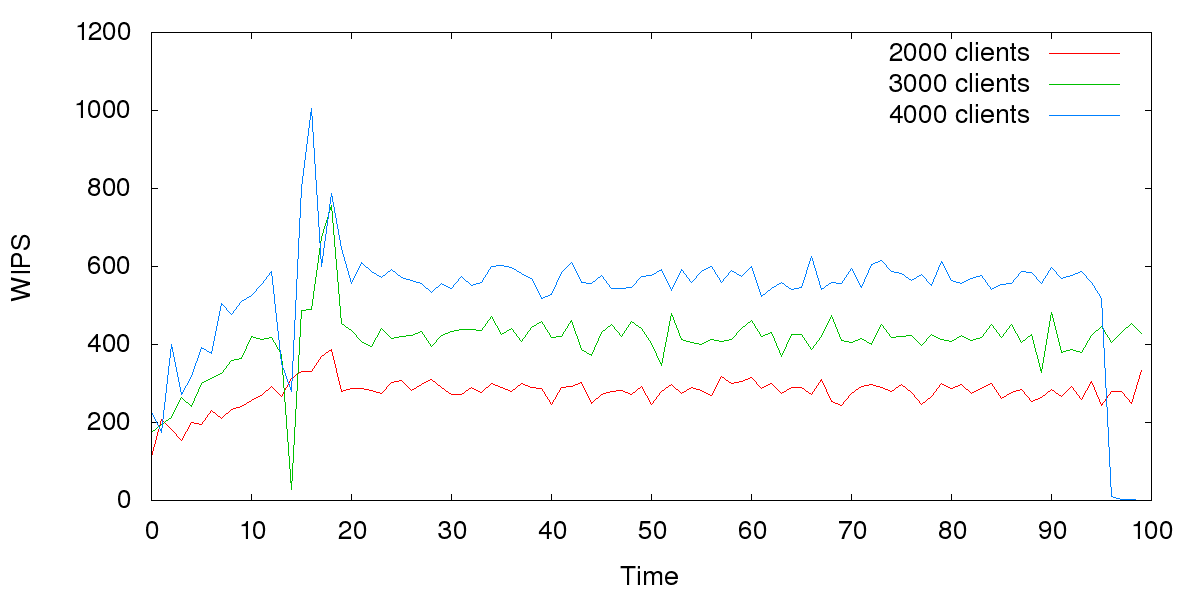
\includegraphics[width=15cm, height=10cm]{images/exp2/plot_browsin}
Figura 4: WIPSb por tempo para cada carga simulada pelo RBE no perfil Browsing no experimento 2
\end{center}

O gráfico indica que um melhor desempenho no geral para 4000 clientes, porém, há uma grande queda no final, que pode indicar problemas devido a alta carga.

\begin{center}
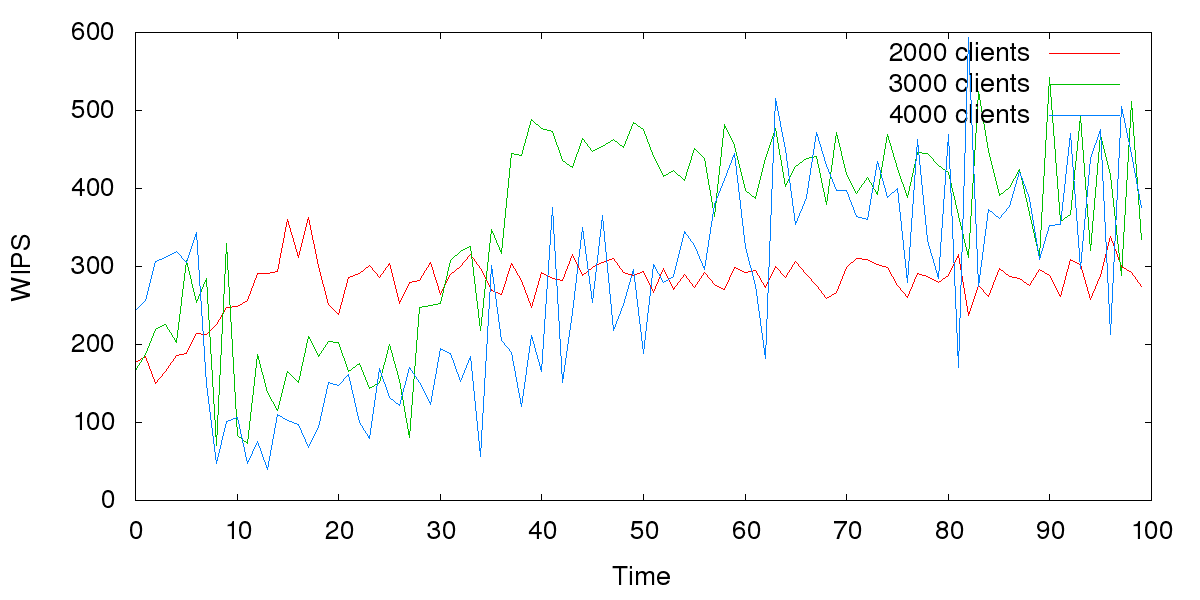
\includegraphics[width=15cm, height=10cm]{images/exp2/plot_ordering}
Figura 5: WIPSo por tempo para cada carga simulada pelo RBE no perfil Ordering no experimento 2
\end{center}

Vemos um melhor desempenho de 3000 clientes no geral, que manteve uma boa média durante todo o experimento e se manteve no mesmo nível de WIPS para 4000 clientes na segunda metade do experimento.

\begin{center}
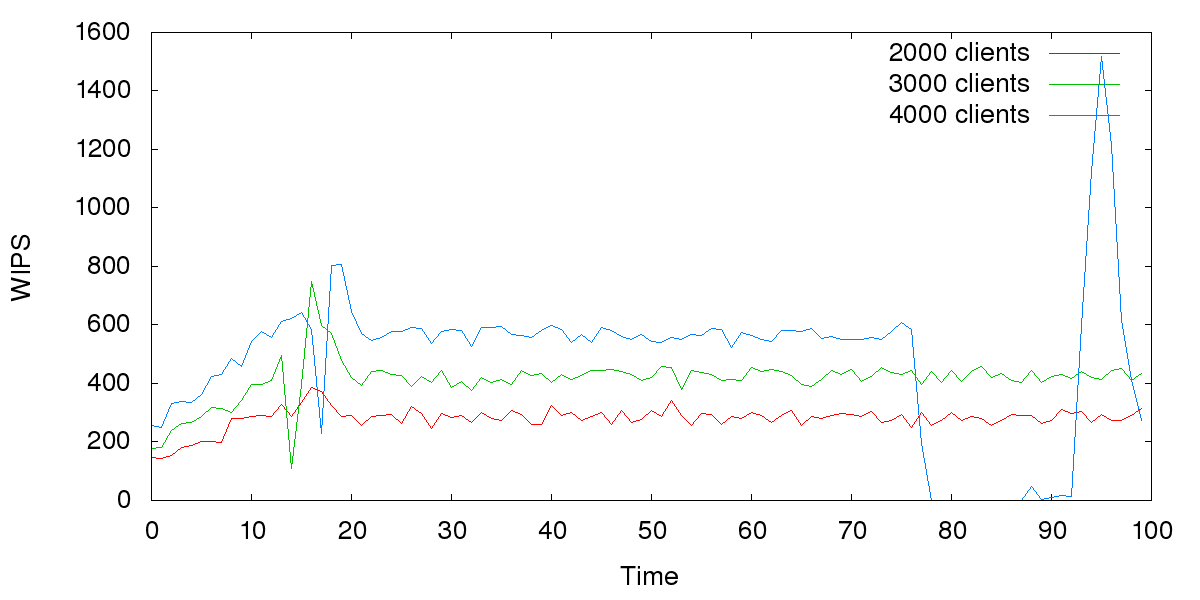
\includegraphics[width=15cm, height=10cm]{images/exp2/plot_shopping}
Figura 6: WIPS por tempo para cada carga simulada pelo RBE no perfil Shopping no experimento 2
\end{center}

Podemos ver que 4000 clientes mantiveram uma taxa de WIPS melhor durante boa parte do experimento, mas existiu uma grande queda dos WIPS na segunda metade, assim como no perfil de Browsing, o que pode indicar que essa carga já está alta e sobrecarregando o servidor.

\section{Conclus\~ao}

\end{document}
